\documentclass[14pt]{extarticle} 
\usepackage{amsmath,mathtools,amsfonts,amsthm,amssymb,hyperref}
\usepackage{wasysym,geometry,bussproofs,latexsym,parskip,bookmark}
\usepackage{mathtools,float}
\newtheorem{defn}{Definition}
\newtheorem{thm}{Theorem}
\newtheorem{claim}{Claim}
\newtheorem{lemma}{Lemma}
\hypersetup{colorlinks,allcolors=blue,linktoc=all}
\geometry{a4paper} 
\geometry{margin=0.5in}
\title{Math for CS 2015/2019 solutions to ``In-Class Problems Week 9, Mon. (Session 21)''}
\author{https://github.com/spamegg1}
\begin{document}
\maketitle
\tableofcontents

\section{Problem 1}
Let $G$ be a $4 \times 4$ grid with vertical and horizontal edges between neighboring vertices. Formally,
$$
V(G) = [0,3]^2 \Coloneqq \{(k, j) \,\, | \,\, 0 \leq k, j \leq 3\}
$$
Letting $h_{i,j}$ be the horizontal edge $\langle (i, j) (i + 1, j\rangle$ and $v_{j,i}$ be the vertical edge $\langle (j, i) (j, i + 1\rangle$ for $i \in [0,2], j \in [0,3]$, the weights of these edges are
$$
w(h_{i,j}) \Coloneqq \frac{4i + j}{100}
$$
$$
w(v_{j,i}) \Coloneqq 1 + \frac{i + 4j}{100}
$$

(A picture of $G$ would help; you might like to draw one.) See below:

\begin{figure}[ht!]
\centering
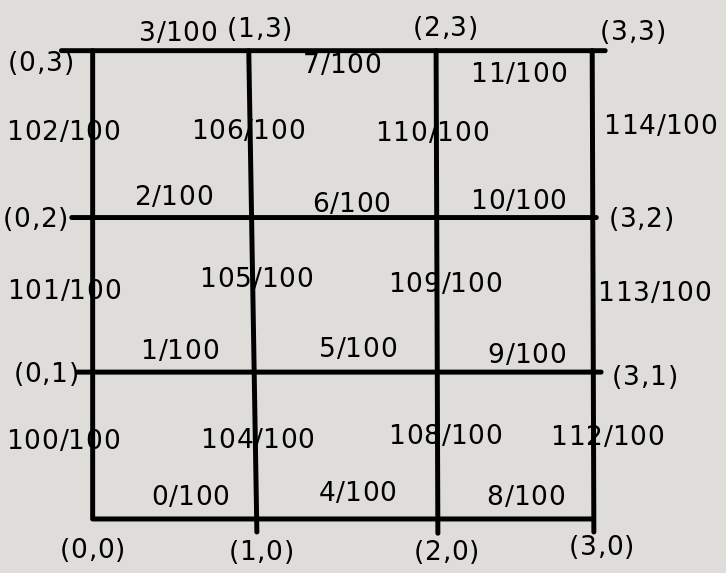
\includegraphics[scale=0.5]{mst-1.png}
\end{figure}

\subsection{(a)}
Construct a minimum weight spanning tree (MST) for $G$ by initially selecting the minimum weight edge, and then successively selecting the minimum weight edge that does not create a cycle with the previously selected edges. Stop when the selected edges form a spanning tree of $G$. (This is Kruskal’s MST algorithm.) Explain how the “gray edge” Lemma 11.10.11 justifies this algorithm in the course textbook.

\begin{proof} See below. The numbers indicate the order of adding edges.
\begin{figure}[ht!]
\centering
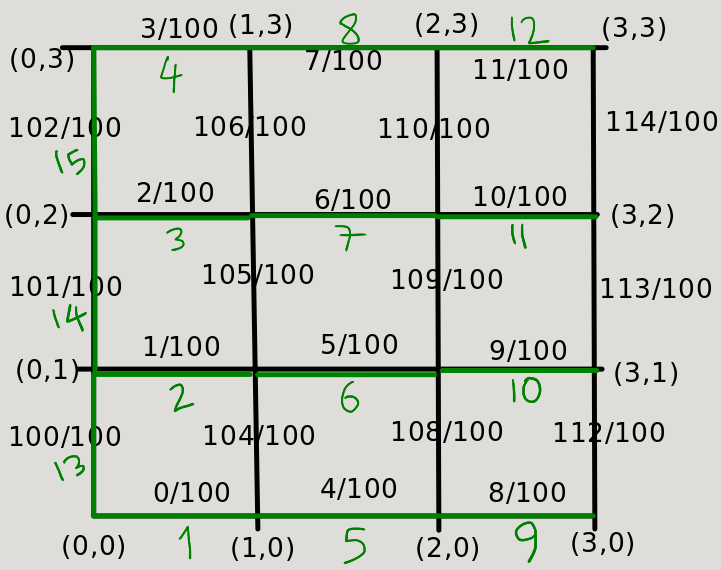
\includegraphics[scale=0.5]{mst-2.png}
\end{figure}
\end{proof}

\subsection{(b)}
Grow an MST for $G$ starting with the tree consisting of the single vertex $(1, 2)$ and successively adding the minimum weight edge with exactly one endpoint in the tree. Stop when the tree spans $G$. (This is Prim’s MST algorithm.) Explain how the “gray edge” Lemma 11.10.11 justifies this algorithm in the course textbook.

\begin{proof} See below. The numbers indicate the order of adding edges.
\begin{figure}[ht!]
\centering
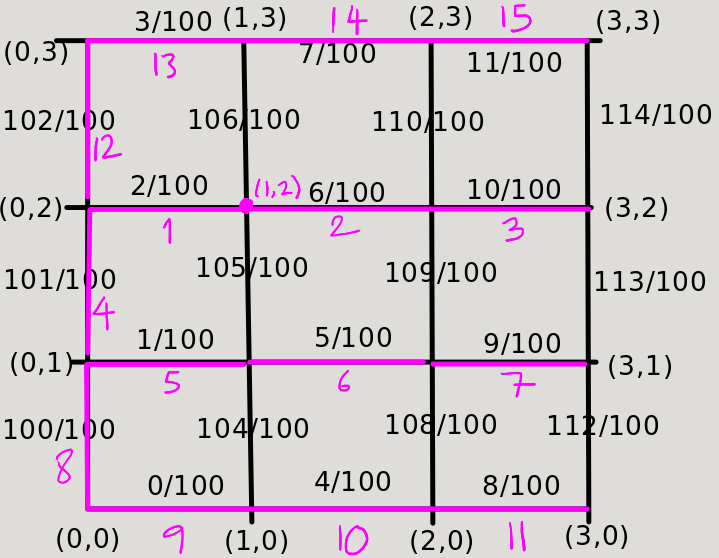
\includegraphics[scale=0.5]{mst-3.png}
\end{figure}
\end{proof}

\subsection{(c)}
Grow an MST for G by treating the vertices $(0,0),(0,3),(2,3)$ as 1-vertex trees and then successively adding, for each tree in parallel, the minimum weight edge among the edges with one endpoint in the tree.

Continue as long as there is no edge between two trees, then go back to applying the general gray edge method until the parallel trees merge to form a spanning tree of $G$. (This is 6.042’s parallel MST algorithm.)

\begin{proof}
See below. The numbers indicate the order of adding edges. The red and blue trees merge after adding 1 edge, and turn into the purple tree. Then the remaining two trees grow up to 6 edges. For the 7th edge we add a gray edge to connect the two separate trees.

\begin{figure}[ht!]
\centering
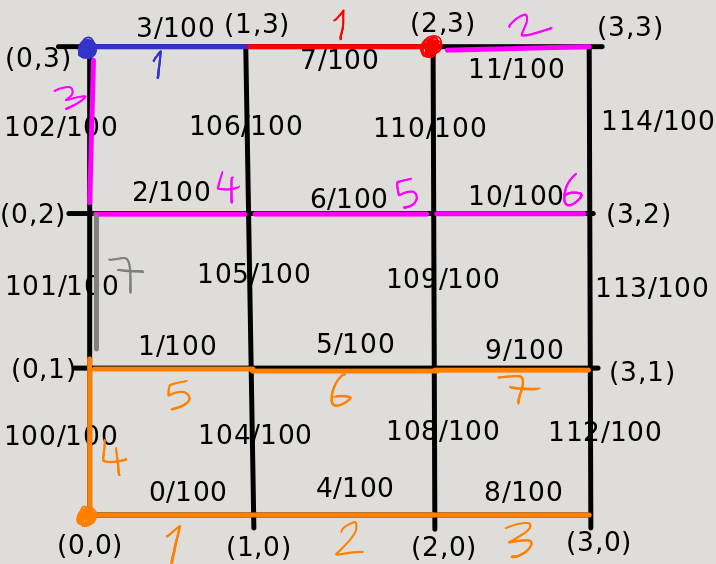
\includegraphics[scale=0.5]{mst-4.png}
\end{figure}
\end{proof}

\subsection{(d)}
Verify that you got the same MST each time.
\begin{proof}
See pictures above.
\end{proof}

\section{Problem 2}
Prove that a graph is a tree iff it has a unique path between every two vertices.

\begin{proof}
Theorem 11.10.3 shows that in a tree there are unique simple paths between any two vertices.

Conversely, suppose we have a graph, $G$, with unique paths. Now $G$ is connected since there is a path between any two vertices. So we need only show that $G$ has no simple cycles. But if there was a simple cycle in $G$, there are two paths between any two vertices on the cycle (going one way around the cycle or the other way around), a violation of uniqueness. So $G$ must cannot have any simple cycles.
\end{proof}

\section{Problem 3}
Let $G$ be a weighted graph and suppose there is a unique edge $e \in E(G)$ with smallest weight, that is, $w(e) < w(f)$ for all edges $f \in E(G) - \{e\}$. Prove that any minimum weight spanning tree (MST) of $G$ must include $e$.

\begin{proof}
1. Assume $M$ is an MST of $G$. Argue by contradiction and assume $M$ does not contain $e$.

2. Say the vertices of $e$ are $v, w$. Since $M$ is a spanning tree, there is a path $p$ in $M$ that starts at $v$ and ends in $w$.

3. Since $e$ is not in $M$, e is not part of the path $p$.

4. Consider $M' \Coloneqq M + e$. Then $M'$ is not a tree, because it now contains a cycle $p + e$ that starts and ends at $v$.

5. Now consider $M'' \Coloneqq M' - f$ where $f \neq e$ is another edge on the path $p$. Notice that $M''$ is a spanning tree.

6. Now consider the weights of $M$ and $M''$:
$$
w(M'') = w(M) + w(e) - w(f) < w(M)
$$
This contradicts the fact that $M$ was a minimum-weight spanning tree (because we constructed another spanning tree $M''$ with less weight).

7. Therefore our assumption in (1) is false, hence $M$ must contain $e$.
\end{proof}

\section{Problem 4}
A simple graph, G, is said to have {\it width w} iff there is a way to list all its vertices so that each vertex is adjacent to at most $w$ vertices that appear earlier in the list. All the graphs mentioned below are assumed to be finite.

\subsection{(a)}
Prove that every graph with width one is a forest.

Hint: By induction, removing the last vertex.

\begin{proof}
Argue by induction on the number $n$ of nodes of a finite simple graph $G$.

{\bf Base Case.} $n = 1$. Assume $G$ is a finite simple graph with $1$ node. So $G$ has no edges, therefore it is a forest.

{\bf Induction Step.} Assume $n \geq 1$ and assume every finite simple graph with $n$ nodes and width one is a forest. Assume $G$ is a finite simple graph with $n+1$ nodes and width one.

Since $G$ has width one, there is a way to list all vertices $v_0, \ldots, v_n, v_{n+1}$ such that each $v_i$ is adjacent to at most 1 vertex that appear earlier in the list.

Consider the graph $G'$ with vertices $\{v_0, \ldots, v_{n+1}\}$ obtained from $G$ by removing $v_{n+1}$ and the only (possible) one edge $e$ between $v_{n+1}$ and one of the previous vertices $v_0, \ldots, v_n$, say $v_j$.

Since $G'$ has $n$ nodes and width 1, by the induction hypothesis $G'$ is a forest. So $G'$ consists of some disconnected trees $T_1', \ldots, T_k'$.

Let $T_i'$ be the tree in $G'$ to which the vertex $v_j$ belongs. Consider the graph $T_i$ obtained from $T_i'$ by adding the edge $e$ and the vertex $v_{n+1}$. Since $v_{n+1}$ is adjacent only to $v_j$, adding the edge $e$ to $T_i'$ does not create a cycle. So $T_i$ is indeed a tree.

This shows that $G$ is a collection of disconnected trees $T_1', \ldots, T_{i-1}', T_i, T_{i+1}', \ldots, T_k$. Therefore $G$ is also a forest.

\end{proof}

\subsection{(b)}
Prove that every finite tree has width one. Conclude that a graph is a forest iff it has width one.

\begin{proof}
Argue by induction on the number $n$ of nodes of a tree.

{\bf Base Case.} $n = 1$. Assume $T$ is a finite tree with $1$ node. In this case we can list the only node, say $v_0$ of $T$. There are no edges, so the adjacency condition is vacuously satisfied.

{\bf Induction Step.} Assume $n \geq 1$ and assume every finite tree with $n$ nodes has width one. Assume $T$ is a finite tree with $n+1$ nodes.

Consider a leaf $l$ of $T$ (a leaf is a ``terminal node'' of a tree, in other words, a node with degree 1). Say $l$ is connected to an internal node $v$ with edge $e$.

Consider the tree $T'$ obtained from $T$ by removing $l$ and $e$. ($T'$ is still a tree, because we only removed a leaf, so it's still connected and cycle-free.)

$T'$ has $n$ nodes. By the induction hypothesis there is a list $v_0, v_1, \ldots, v_n$ of all the nodes of $T'$ such that each node is adjavent to at most 1 node earlier in the list.

Now consider the list of nodes $v_0, \ldots, v_n, l$ of $T$. We know that $l$ is adjacent to exactly one node $v$, which is earlier in the list, among the $v_0, \ldots, v_n$. Therefore $T$ also has width 1. This finishes the proof of the Induction Step.

By the Principle of Mathematical Induction, every finite tree has width 1.

For the second claim:

Assume a finite simple graph $G$ is a forest. So $G$ is a collection of disconnected finite trees $T_1, T_2, \ldots, T_n$. By part (b) each $T_i$ has width 1. Since the trees are disconnected, it follows that $G$ also has width 1.

Conversely assume a finite simple graph $G$ has width 1. By part (a) $G$ is a forest.
\end{proof}
\end{document}
